\section{Shrinkage Properties of the $\mathrm{QVP}$} \label{sec:theoretical-properties}
In this section, we analyse the $\QVP$ prior in terms of its implications on the shrinkage scale space. It is common to analyse global-local priors in terms of their implied distribution on a scale that allows to gauge the shrinkage effect away from the maximum likelihood estimate \citep{polson_half-cauchy_2012}.  As is common in the literature, we analyse the shrinkage scale distribution for the normal model.\footnote{Derivations can be extended to the $\mathcal{ALD}$ using the shrinkage coefficient definitions in \citet{kohns2024horseshoe}} Applied to an isotropic normal observation model, we define fused shrinkage akin to the $\QVP$ in the following model structure: 
%
\begin{IEEEeqnarray}{rl}
    y_t & = x_t^T\beta_t + \epsilon_t, \quad \epsilon_t \sim \normal\left(0,\sigma_{y}^2\right) \\
    \beta_t & \sim \normal\left(\beta_{t-1},\nu^2\Lambda_t\right),\; \Lambda_t = \mathrm{diag}\left( \lambda_{t,1}^2,\dotsc, \lambda_{t,K}^2 \right) \\
    \beta_t\vert \beta_{1},\dotsc,\beta_{t-1},y,\vartheta \; & \propto \normal\left(\overline{\beta}_t,K_{\beta_t}^{-1}\right).
\end{IEEEeqnarray}
%
$K_{\beta_t} = (\nu^{-2}\Lambda_t^{-1} + \frac{1}{\sigma_y^2}x_t^Tx_t)$ and $\overline{\beta}_t = K^{-1}_{\beta_t}\left(\nu^{-2}\Lambda_t^{-1}\beta_{t-1} + \frac{1}{\sigma_y^2}x_t^Ty_t\right)$ where $\beta_t \in \mathbbm{R}^{K}$. Assume further that $x_t^Tx_t \approx \mathrm{diag}(1,\dotsc,1)$, then the posterior mean can be further decomposed as:
%
\begin{equation}
    \kappa_{t,j} \beta_{t-1,j} + (1-\kappa_{t,j})\beta_{\mathrm{ML},t,j},
\end{equation}
%
where $\kappa_{t,j} = \frac{1}{\nu^2\lambda_{t,j}^2\sigma^{-2}_y+1}$ and $\beta_{\mathrm{ML},t,j} = \left(x_{t,j}\right)^{-2}x_{t,j}y_t$ can be understood as a maximum likelihood esimate to the coefficient $\beta_{t,j}$.
%
This decomposition shows that the conditional posterior mean is a convex combination of the prior coefficient $\beta_{t-1}$ and a maximum likelihood estimate. Therefore, as $\lambda^2_{t,j}\rightarrow0$, then $\kappa_{t,j}\rightarrow1$ and $(1-\kappa_{t,j})\rightarrow 0$. Hence, with strong shrinkage toward the origin, there is no further updating implied from the data, and the posterior concentrates on the previous coefficient $\beta_{t-1,j}$. On the other-hand when $\lambda^2_{t,j}\rightarrow\infty$, then $\kappa_{t,j} \rightarrow0$ and $(1-\kappa_{t,j})\rightarrow1$, so updating the posterior only happens with the data information at observation $t$, and the previous coefficient has no further influence. 
%
\begin{definition}\label{eq:def-1}
    Suppose $\lambda_{t,j}\sim C_+(0,1)$, then the probability density function of the shrinkage coefficient $\kappa_{t,j}$, conditional on $(\nu,\sigma_y)$ can be shown to be
    \begin{equation}
        p(\kappa_{t,j}\vert \nu,\sigma_y) = \frac{1}{\pi}\frac{\nu\sigma^{-1}_y}{(\nu^2\sigma^{-2}_y-1)\kappa_{t,j}+1}\frac{1}{\sqrt{\kappa_{t,j}}\sqrt{1-\kappa_{t,j}}},
    \end{equation}
    which is proportional to $\betadist(1/2,1/2)$ when $\nu \sigma_y=1$.
\end{definition}
%
See Appendix~\ref{sec:shrinkage-properties} for further derivations. The implied prior distribution for $\kappa_{t,j}$ is shown in Figure~\ref{fig:ShrinkageCoefficients}. Hence, shrinkage properties that are well understood for the prior on levels of coefficients also transfer to difference shrinkage. The Cauchy prior on $\lambda_{t,j}$ results in a continuous approximation to variable selection type behaviour: probability density is highest on strong or very little shrinkage respectively.
\begin{figure}
    \centering
    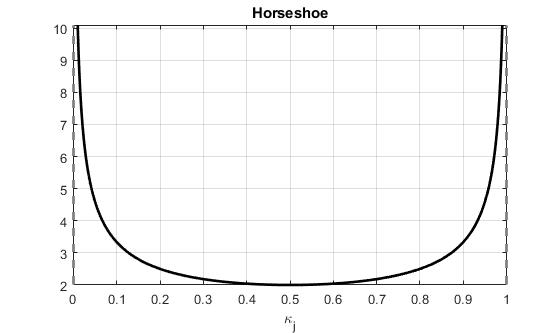
\includegraphics[width=\textwidth]{Figures/HS_kappa.jpg}
    \caption{Distribution of $\kappa_{t,j}$, the shrinkage coefficient implied by the horseshoe prior.}
    \label{fig:ShrinkageCoefficients}
\end{figure}
%
